\documentclass[../main.tex]{subfiles}

\begin{document}
	\section{Vorgehen / Methoden}
	
	\subsection{Swagger}
	Erste Umsetzungen finden mithilfe eines Swaggerprojekts statt. Hier kann ein Entwurf erstellt werden. Mithilfe dieses Entwurfs wird ein Grundgerüst hergestellt, welcher dazu dient, vereinfacht die REST Schnittstelle zu bauen.
	
	\begin{figure}[H]
		\centering
		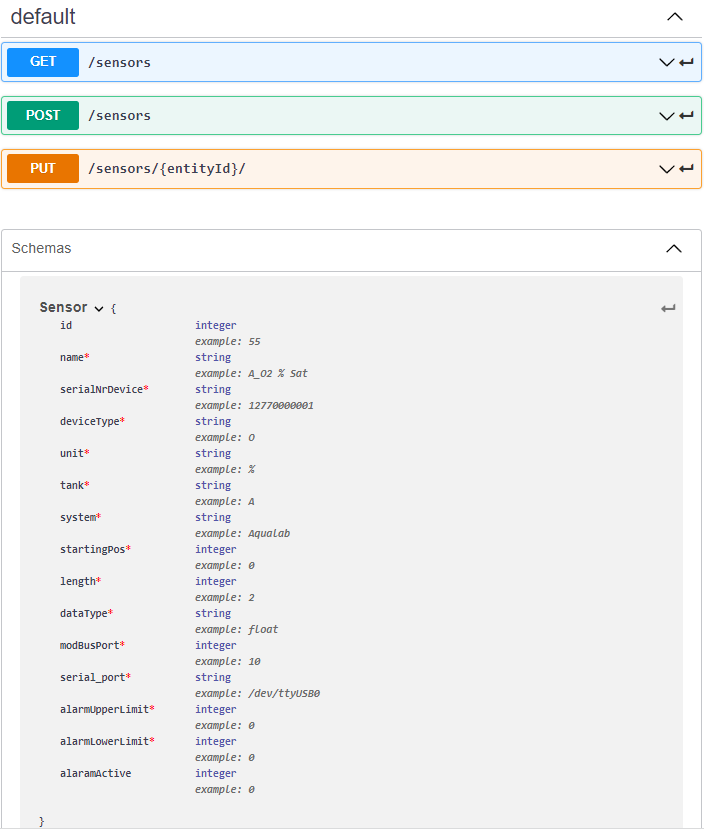
\includegraphics[scale=0.4]{Swagger}
		\caption{Swagger Beispiel}
		\label{fig:Swagger}
	\end{figure}
	\par
	\noindent
	Die Schnittstelle soll dazu fähig sein Daten der Sensoren zurückzugeben. Die Möglichkeit soll bestehen, dass die Sensorendaten zusätzlich editierbar sind.\\
	\\
	Als Vereinfachung können die Sensoren auch als eine Liste angezeigt werden.
	
	\subsection{Continuous Integration}
	Als Source Control wird Git eingesetzt und um mit allen Entwicklern zusammen zu arbeiten befindet sich das Repository auch auf github.com. Github bietet uns mit den Github Actions ein gutes Tool welches wir automatisch das gesamte Spring-Boot Projekt erstellen, testen und auf DockerHub hochladen können. Die Github Actions werden bei jedem Push in den Main Branch angestossen. In den Main Branch wird in der Regel nur dann gepusht wenn ein Feature Branch nach Pull Request und Code Review in den Main gemergerd wird. Daher wird das Github Actions nicht bei jedem Commit ausgeführt und nur funktionierende Versionen werden auf Dockerhub hochgeladen.
	
	\begin{lstlisting}[language=yaml]
		# This is a basic workflow to help you get started with Actions
		
		name: CI to Docker Hub
		
		# Controls when the workflow will run
		on:
		# Triggers the workflow on push or pull request events but only for the main branch
		push:
		branches: [ main ]
		pull_request:
		branches: [ main ]
		
		# Allows you to run this workflow manually from the Actions tab
		workflow_dispatch:
		
		# A workflow run is made up of one or more jobs that can run sequentially or in parallel
		jobs:
		# This workflow contains a single job called "build"
		build:
		# The type of runner that the job will run on
		runs-on: ubuntu-latest
		
		# Steps represent a sequence of tasks that will be executed as part of the job
		steps:
		# Checks-out your repository under $GITHUB_WORKSPACE, so your job can access it
		- name: Checkout Repo
		uses: actions/checkout@v2
		
		# Gradle Build
		- name: Set up JDK 11
		uses: actions/setup-java@v2
		with:
		java-version: '11'
		distribution: 'adopt'
		- name: Validate Gradle wrapper
		uses: gradle/wrapper-validation-action@e6e38bacfdf1a337459f332974bb2327a31aaf4b
		- name: Build with Gradle
		run: ./gradlew bootJar
		
		# Login to Docker Hub
		- name: Login to Docker Hub
		uses: docker/login-action@v1
		with:
		username: ${{ secrets.DOCKER_HUB_USERNAME }}
		password: ${{ secrets.DOCKER_HUB_ACCESS_TOKEN }}
		
		# Set up Docker Buildx
		- name: Set up Docker Buildx
		id: buildx
		uses: docker/setup-buildx-action@v1
		
		# Build and push
		- name: Build and push
		id: docker_build
		uses: docker/build-push-action@v2
		with:
		context: ./
		file: ./Dockerfile
		push: true
		tags: ${{ secrets.DOCKER_HUB_USERNAME }}/paaq:latest
		
		# Image digest
		- name: Image digest
		run: echo ${{ steps.docker_build.outputs.digest }}
	\end{lstlisting}
	
	\subsection{Docker}
	Docker kann sehr vielfältig eingesetzt werden, aber worin Docker seine stärken hat ist im Deployment. Mit einem gutem Docker-Compose File ist ein komplexes Multi-Container System mit einem Befehl aufgesetzt.
	
	\subsubsection{Docker-Image}
	Von unserer Spring-Boot Applikation erstellen wir ein Image welches auf DockerHub hochgeladen wird. Von der Datenbank erstellen wir kein Image da DockerHub wie Github öffentlich zugänglich ist und wir die Datenbank nicht veröffentlichen wollen. Die Datenbank wird dann beim erstellen des MySQL Containers eingelesen wie im nächsten Abschnitt erklärt.
	
	\subsubsection{Docker-Compose}
	Das Docker-Compose holt sich die neuste Version der Applikation und erstellt ein Netzwerk für das Gesamte PAAQ-System. Der Applikation wird ein Portforwarding eingerichtet, dass diese auch von Aussen zugänglich ist. Anschliessend wird auch ein MySQL-Container heruntergeladen und in das gleiche Netzwerk eingehängt, dass eine Kommunikation zwischen Spring-Boot Applikation und MySQL-Datenbank statt finden kann. Der MySQL Datenbank wird noch der Dump der alten Datenbank mitgegeben, dass eine exakte Kopie der vorherigen Datenbank erstellt.
	\begin{lstlisting}[language=yaml]
		version: "3.3"
		
		services:
		  mysqldb:
		    image: mysql:latest
		    container_name: mysqldb_aquaponics
		    restart: unless-stopped
		    environment:
		      - MYSQL_ROOT_PASSWORD=[MYSQL_ROOT_PASSWORD]
		      - MYSQL_DATABASE=[MYSQL_DATABASE]
		    ports:
		      - "3306"
		    volumes:
		      - /home/[user]/dump:/docker-entrypoint-initdb.d
		      
		  spring_boot:
		    image: [dockerhub_username]/paaq:latest
		    container_name: spring_boot_aquaponics
		    restart: on-failure
		    ports:
		      # map port 8080 on host to 8080 on container
		      - "8080:8080"
	\end{lstlisting}

	\subsection{Gesamtsystem}
	Auf dem folgendem Bild ist das gesamte System abgebildet, welches bei Hetzner gehostet wird.
	\begin{figure}[h]
		\centering
		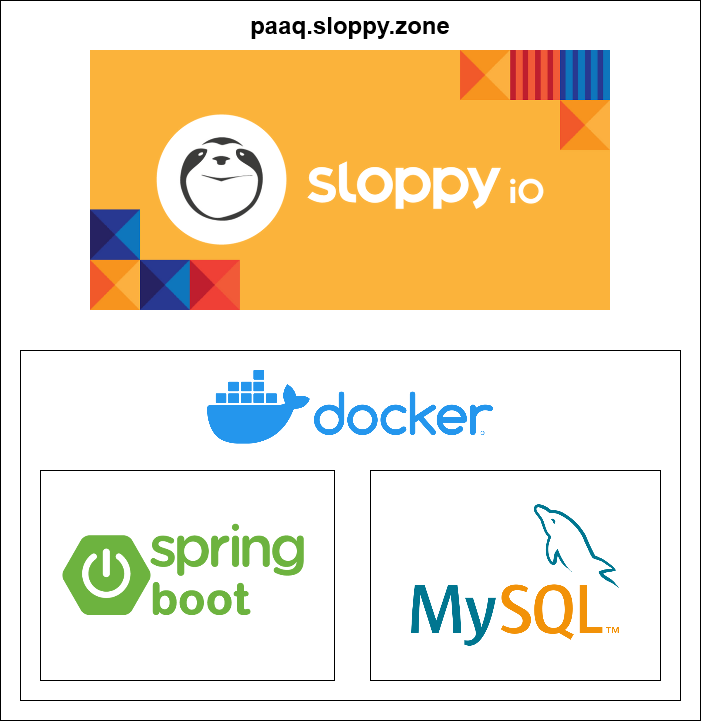
\includegraphics[scale=0.4]{pa_aquaponics_docker_architecture}
		\caption{Gesamtsystem}
		\label{fig:Gesamtsystem}
	\end{figure}
	
\end{document}